\section{Approach}
\subsection{Simulated Network}

The network of our simulation is designed to give a real-time nature to the data transfer between the Tennessee Eastman(TE) physical simulation and the TE Controller. Both the controller and simulation are written in Matlab and connected to our network with the OMNeTBridge Class. (These are described in later sections.)

The network is based primarily on two factory level components, sensors and actuators, that send data to a remote facility that sends back control signals. This is based on most SCADA systems that need remote facilities to monitor their data. These signals are sent over a simulated "Internet" that allows accurate packet loss, bit errors and data rates. 

Due to limitations of the default Inet packets we are not actually sending the data through the network. Rather, the packets the controller receives act as a trigger to have the controller update the data from that sensor, and send an update to the actuators if need be. 

The actual implementation of these components is described in later sections. 


\subsection{Controller}


\subsubsection{Actuator}

The actuator acts as a server which receives an update packet from the controller, grabs its appropriate data from the controller OMNeTBridge and then passes it to the correct function.

\subsubsection{Sensor}


The Sensor is a relatively simple module that sends an update signal based on a timer. This is to model the refresh rate of most sensors. We have assumed that all sensors and network controllable and are able to tirelessly connect to a local access point via 802.11 Wireless LAN(WiFi). 

These modules send a TCP packet to a known IP address which in turn triggers the controller to update. This is a non-ideal method of updating as it does not allow correct implementation of attacking the data on the network. Ideally INET's TCP packets would allow us to send data to them, however as some modules are currently implemented deep copies are not done of messages or inappropriate casts are used. Future work should be planned to modify these modules or find a more correct
implementation of INET messages that allow custom data fields to be created and sent. 

\subsubsection{Internet Cloud}

\subsubsection{Factory Access Point}

\subsubsection{Factory Bridge}

\subsection{Matlab Simulation}
 We chose to use MATLAB simulation for the physical system and it's controls, as there are many chemical process models currently implemented in MATLAB. This allows for the ease of swapping out current MATLAB models for new ones.

\subsubsection{Tennessee Eastman}
 In order to keep the complexity down, we decided to model the chemical process in the plant as a simplified Tennessee Eastman problem\citation{Ricker}. Due to this approach, we looked to previous work in the field, and found many models already modeled in a hybrid of FORTRAN and MATLAB.  However, this introduced more complexity, due to using three different programming languages to implement what should be simpler.  Therefore, we would build a custom MATLAB class that contained the same functionality.  This includes a both the simulation of the actual Tennessee Eastman system, and the steady state controller calculations.


\subsection{C++ to Matlab Bridge}

In order to connect the two models implemented in MATLAB and OMNeT++, a bridge was implemented using standard TCP sockets. Both sides implement classes which makes communicating with the simulation running on the other program easy to interface with. Packets in the form of strings are sent back and forth. These packets contain a header and a variable number of data values. Each data value has a name as a string, a type, and a value (the actual representation of which depends on the type). The supported types are integers, floats and strings, with doubles being partially implemented. However, as the Tennessee-Eastman simulation only used integers and floats, only these types have been significantly tested. Both sides parse the packets into their respective language representations to allow for easier use.

On the MATLAB side, a MATLAB class, OMNeTPipe, is used to establish a connection and send and receive packets. In the constructor for this class, a TCP server socket is opened on a specified port. Once connected to OMNeT++, the pipe can be used to send and receive packets, where the receive function is blocks until a full packet is received. Once a packet string is received, the string is parsed and the header is returned as a string with the data values stored as a map, with the variable name used as the key. When sending a packet, the send function takes in a variable number of arguments, where the header and data names, types and values are passed into the function. These are then formed into a string and written to the socket. The send function is non-blocking.

On the OMNeT++ side, a few C++ classes are used to complete the interface. The first, OMNeTPipe, mirrors the MATLAB side, which, in the constructor, attempts to connect a TCP socket to a given port and host. A socket exception is thrown on failure. The socket interface for the C++ side was borrowed from Jeff Donahoo's PracticalSocket class from Baylor University School of Engineering and Computer Science. Once a connection is established, similar send and receive functions can be used to transfer values to and from MATLAB. However, the C++ interface also uses another class to make the storage of packets more convenient. The OMNeTPk class is used to store values to be sent and received from MATLAB. Thus, the send function takes in a pointer to one of these objects, and the received function returns a pointer to an OMNeTPk object. These objects allow values to be set with the addVal function and values to be retrieved by name. Internally, the OMNeTPk stores values, names and types in C++ vectors, using void* generic values to store the integers, floats and strings supported by the pipe interface. Thus, similar to the MATLAB map, the variables can be retrieved via their names associatively.

In order to better facilitate communication between OMNeT++ and MATLAB in the Tennessee-Eastman simulation, another C++ class was implemented. The OMNeTBridge class is a more project-specific class which holds the various control and feedback variables from the MATLAB simulation for the various OMNeT++ network objects to use. This class uses the OMNeTPipe to connect to MATLAB to send and received data and store it locally. Thus, a system state is maintained in both MATLAB and OMNeT++. On the system side, a bridge connects the MATLAB Tennessee-Eastman simulation to the sensors and actuators. On the controller side, a separate bridge connects the MATLAB controller model to the controller network application. In the constructor of the bridge, an OMNeTPipe is opened depending on the type of the bridge (controller or system side). Once established, an UPDATE packet is sent. This packet consists of an id (always 1) and a dt value. OMNeT++ is used to keep time, thus all packets sent to MATLAB contain this change in time so the MATLAB model can update itself appropriately. MATLAB, after updating the model, sends back a STATUS packet containing s the current settings for all 14 variables. The bridge then stores these values. The bridge also provides methods to set and request parameters from the MATLAB model. When requesting data, the bridge sends MATLAB an UPDATE packet with the time change since the last packet was sent over the bridge and then waits for the STATUS response. Once received, the bridge updates its internal state and returns the requested value to caller (being a sensor or the controller). In the case of a setVal call, the bridge sends a CHANGE packet, which includes the information from an UPDATE packet with whatever parameters are to be set to the given values. Once sent, a STATUS packet is received to update the internal state of the bridge. Depending on the bridge type, either control parameters (for actuators) or status parameters (for the controller) are sent. This bridge object makes interfacing MATLAB and OMNeT++ simulations quick and straightforward.


\begin{figure*}
        \centering
		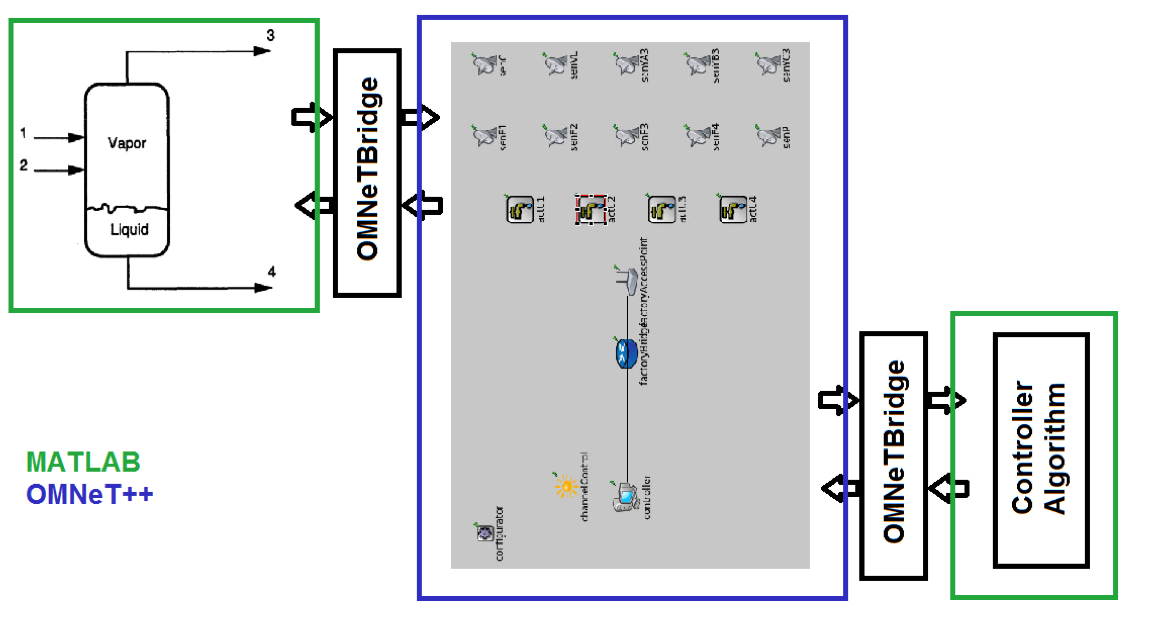
\includegraphics[width=0.8\textwidth]{figs/system.png}
        \caption{System Diagram.}
        \label{fig:system}        
\end{figure*}
